\let\negmedspace\undefined
\let\negthickspace\undefined
\documentclass[journal]{IEEEtran}
\usepackage[a5paper, margin=10mm, onecolumn]{geometry}
%\usepackage{lmodern} % Ensure lmodern is loaded for pdflatex
\usepackage{tfrupee} % Include tfrupee package

\setlength{\headheight}{1cm} % Set the height of the header box
\setlength{\headsep}{0mm}     % Set the distance between the header box and the top of the text

\usepackage{gvv-book}
\usepackage{gvv}
\usepackage{cite}
\usepackage{amsmath,amssymb,amsfonts,amsthm,mathtools}
\usepackage{algorithmic}
\usepackage{graphicx}
\usepackage{textcomp}
\usepackage{xcolor}
\usepackage{txfonts}
\usepackage{listings}
\usepackage{enumitem}
\usepackage{mathtools}
\usepackage{gensymb}
\usepackage{comment}
\usepackage[breaklinks=true]{hyperref}
\usepackage{tkz-euclide} 
\usepackage{listings}
\def\inputGnumericTable{}                                 
\usepackage[latin1]{inputenc}                                
\usepackage{color}                                            
\usepackage{array}                                            
\usepackage{longtable}                                       
\usepackage{calc}                                             
\usepackage{multirow}                                         
\usepackage{hhline}                                           
\usepackage{ifthen}                                           
\usepackage{lscape}
\begin{document}

\bibliographystyle{IEEEtran}
\vspace{3cm}

\title{1.8.19}
\author{EE24BTECH11002 - Agamjot Singh}
% \maketitle
% \newpage
% \bigskip
{\let\newpage\relax\maketitle}
%\newcommand{\norm}[1]{\abs{\abs{#1}}}
\renewcommand{\thefigure}{\theenumi}
\renewcommand{\thetable}{\theenumi}
\setlength{\intextsep}{10pt} % Space between text and floats

\textbf{Question:}
\newline
Find the points on $X$ axis which are at a distance of $2\sqrt{5}$ from the point \brak{7, -4}. How many such points are there?
\newline
\textbf{Solution:}
\newline
Let $\vec{A}$ $\myvec{7\\-4}$ and $\vec{B} \myvec{x\\y}$ be the desired point on the $X$ axis.
\newline
The $L_p$ norm, written as $\norm{x}_p$, is defined as
\begin{align}
	\norm{x}_p = \sqrt[p]{\sum_{i=1}^{n}\abs{x_i}^p}, p\geq 1
\end{align}
If $\vec{B}$ is at a distance of $2\sqrt{5}$ from point $\vec{A}$.
\begin{align}
	\norm{\vec{B} - \vec{A}}_p &= 2\sqrt{5}\\
	\implies \sqrt[p]{\abs{x - 7}^p + \abs{y + 4}^p} &= 2\sqrt{5}\\
\end{align}
Taking $y = 0$, as $\vec{B}$ lies on the $X$ axis.
\begin{align}
	\sqrt[p]{\abs{x - 7}^p + \abs{4}^p} &= 2\sqrt{5}\\
	\abs{x - 7}^p + \brak{4}^p &= \brak{2\sqrt{5}}^p\\
	\abs{x - 7} &= \sqrt[p]{\brak{2\sqrt{5}}^p - \brak{4}^p}\\
	x &= 7 \pm \sqrt[p]{\brak{2\sqrt{5}}^p - \brak{4}^p}
\end{align}

By solving equation \brak{7} with $y = 0$, we get,
\begin{align}
	\vec{B} = \myvec{7 \pm \sqrt[p]{\brak{2\sqrt{5}}^p - \brak{4}^p}\\0}, p \geq 1 
\end{align} 
There are infinitely many such points as $p$ varies from $1$ to $\inf$.

\begin{figure}[h!]
   \centering
   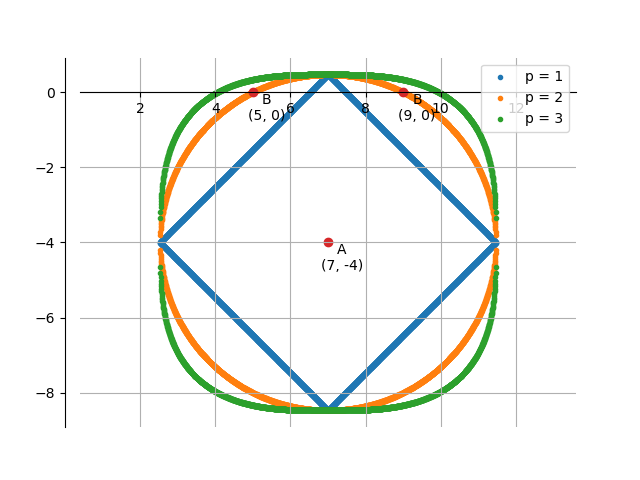
\includegraphics[width=0.7\linewidth]{figs/graph.png}
   \caption{Graph representing the locus of $\vec{B}$, taking $p = 1, 2, 3$}
\end{figure}

\end{document}
